\documentclass[border=10pt]{standalone}
% Shared style for the EMONI diagrams. Build: tectonic <file>.tex, then pdftocairo -svg.
\usepackage{fontspec}
\setmainfont{FiraSans}[Extension=.otf,UprightFont=*-Regular,BoldFont=*-SemiBold,ItalicFont=*-Italic,BoldItalicFont=*-SemiBoldItalic]
\setmonofont{FiraMono}[Extension=.otf,UprightFont=*-Regular,BoldFont=*-Medium,Scale=0.9]
\usepackage{tikz}
\usetikzlibrary{arrows.meta,positioning,shapes.geometric,shapes.misc,calc,fit,backgrounds}
\definecolor{eg}{HTML}{11903B}   % EMONI green
\definecolor{egl}{HTML}{E8F7EE}
\definecolor{eb}{HTML}{2A78D6}   % blue
\definecolor{ebl}{HTML}{EAF2FC}
\definecolor{eo}{HTML}{D9631E}   % orange
\definecolor{eol}{HTML}{FDF0E7}
\definecolor{ep}{HTML}{7C4DCC}   % purple
\definecolor{epl}{HTML}{F2ECFB}
\definecolor{er}{HTML}{C5221F}   % red
\definecolor{erl}{HTML}{FCEAEA}
\definecolor{ink}{HTML}{1F2328}
\definecolor{mute}{HTML}{59636E}
\definecolor{line}{HTML}{D0D7DE}
\tikzset{
  every node/.style={text=ink,font=\small},
  >={Stealth[length=2.4mm]},
  % sequence diagrams
  life/.style={draw=line,dashed,thick},
  head/.style={draw=#1,fill=#1!8,rounded corners=3pt,minimum width=27mm,minimum height=11mm,align=center,font=\small\bfseries,thick},
  act/.style={draw=#1,fill=#1!18,minimum width=2.2mm},
  msg/.style={->,thick,draw=ink},
  ret/.style={->,dashed,draw=mute},
  mlabel/.style={font=\footnotesize,fill=white,inner sep=1.5pt,align=center},
  note/.style={draw=#1,fill=#1!8,rounded corners=2pt,font=\footnotesize,align=left,inner sep=4pt},
  frag/.style={draw=mute,rounded corners=2pt},
  fraglabel/.style={draw=mute,fill=white,font=\footnotesize\bfseries,inner sep=2.5pt,anchor=north west},
  % activity diagrams
  start/.style={circle,fill=ink,minimum size=4mm,inner sep=0},
  stop/.style={circle,draw=ink,thick,minimum size=5mm,inner sep=0,path picture={\fill[ink] (path picture bounding box.center) circle (1.4mm);}},
  step/.style={draw=#1,fill=#1!8,rounded corners=5pt,thick,minimum height=9mm,minimum width=40mm,align=center,font=\small},
  step/.default=eg,
  dec/.style={diamond,aspect=2.2,draw=ink,fill=white,thick,inner sep=1.5pt,align=center,font=\footnotesize},
  flow/.style={->,thick,draw=ink},
  guard/.style={font=\footnotesize\itshape,text=mute,fill=white,inner sep=1.5pt},
  lane/.style={draw=line,fill=#1,rounded corners=4pt},
  lanetitle/.style={font=\small\bfseries,text=mute},
}

% Activity: a connectivity test plan run by the test host against a live device.
\begin{document}
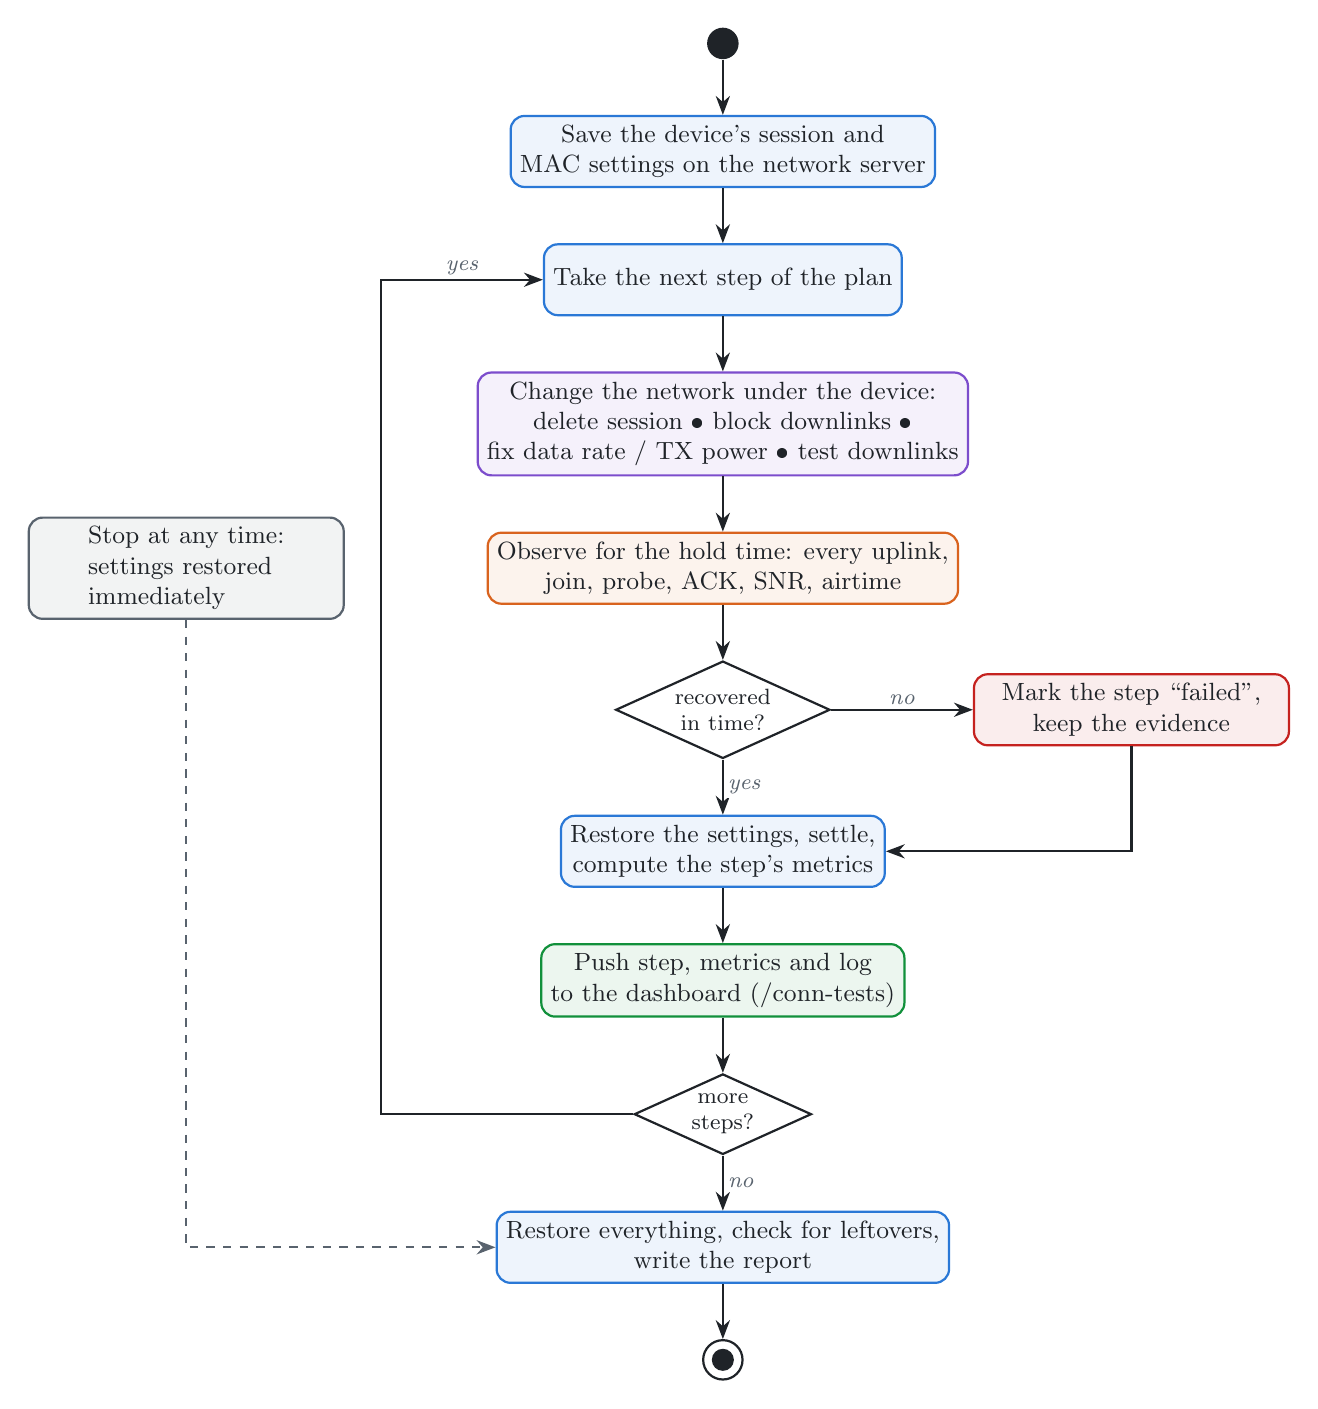
\begin{tikzpicture}[node distance=7mm and 14mm]
\node[start] (s) {};
\node[step=eb,below=of s] (save) {Save the device's session and\\MAC settings on the network server};
\node[step=eb,below=of save] (next) {Take the next step of the plan};
\node[step=ep,below=of next] (apply) {Change the network under the device:\\delete session \textbullet{} block downlinks \textbullet{}\\fix data rate / TX power \textbullet{} test downlinks};
\node[step=eo,below=of apply] (obs) {Observe for the hold time: every uplink,\\join, probe, ACK, SNR, airtime};
\node[dec,below=of obs] (rec) {recovered\\in time?};
\node[step=eb,below=of rec] (rest) {Restore the settings, settle,\\compute the step's metrics};
\node[step=eg,below=of rest] (push) {Push step, metrics and log\\to the dashboard (/conn-tests)};
\node[dec,below=of push] (more) {more\\steps?};
\node[step=eb,below=of more] (fin) {Restore everything, check for leftovers,\\write the report};
\node[stop,below=of fin] (e) {};
\node[step=er,right=18mm of rec] (bad) {Mark the step ``failed'',\\keep the evidence};
\node[step=mute,left=18mm of obs,align=left] (stop) {Stop at any time:\\settings restored\\immediately};
\draw[flow] (s)--(save); \draw[flow] (save)--(next); \draw[flow] (next)--(apply);
\draw[flow] (apply)--(obs); \draw[flow] (obs)--(rec);
\draw[flow] (rec)--node[guard,right]{yes}(rest);
\draw[flow] (rec)--node[guard,above]{no}(bad);
\draw[flow] (bad.south) |- (rest.east);
\draw[flow] (rest)--(push); \draw[flow] (push)--(more);
\draw[flow] (more)--node[guard,right]{no}(fin); \draw[flow] (fin)--(e);
\draw[flow] (more.west) -- ++(-3.2,0) |- node[guard,above,pos=0.75]{yes} (next.west);
\draw[flow,dashed,draw=mute] (stop.south) |- (fin.west);
\end{tikzpicture}
\end{document}
